% Minimal wrapper to test-compile architecture_diagram.tex as a standalone PDF.
\documentclass[11pt]{article}
\usepackage[margin=0.4in,letterpaper]{geometry}
\usepackage[T1]{fontenc}
\usepackage{lmodern}
\usepackage{xcolor}
\usepackage{tikz}
\usetikzlibrary{shapes.geometric, arrows.meta, positioning, calc, fit, backgrounds, shadows}

% --- Colors ---
\definecolor{agentOrange}{RGB}{255, 240, 220}
\definecolor{agentCyan}{RGB}{225, 250, 250}
\definecolor{agentPurple}{RGB}{240, 230, 255}
\definecolor{agentTeal}{RGB}{220, 245, 245}
\definecolor{googleGray}{RGB}{240, 240, 240}
\definecolor{orchBlue}{RGB}{230, 240, 255}
\definecolor{planGreen}{RGB}{235, 255, 235}
\definecolor{failRed}{RGB}{255, 220, 220}
\definecolor{stateBlue}{RGB}{235, 245, 255}

% --- Icons ---
\newcommand{\iconDNA}[1]{\tikz[baseline=-3pt, scale=0.25]{\draw[#1, thick] (0,0) sin (0.5,0.5) cos (1,0) sin (1.5,-0.5) cos (2,0);\draw[#1, thick] (0,0) sin (0.5,-0.5) cos (1,0) sin (1.5,0.5) cos (2,0);}}
\newcommand{\iconGraph}[1]{\tikz[baseline=-3pt, scale=0.25]{\fill[#1] (0,0) circle (5pt) (1,0.5) circle (5pt) (1,-0.5) circle (5pt);\draw[#1, thick] (0,0)--(1,0.5) (0,0)--(1,-0.5) (1,0.5)--(1,-0.5);}}
\newcommand{\iconSearch}[1]{\tikz[baseline=-3pt, scale=0.25]{\draw[#1, thick] (0,0) circle (0.5cm);\draw[#1, very thick] (0.35,-0.35)--(0.7,-0.7);}}
\newcommand{\iconBulb}[1]{\tikz[baseline=-3pt, scale=0.25]{\draw[#1, thick, fill=white] (0,0) circle (0.5cm);\draw[#1] (-0.2,-0.4)--(-0.2,-0.7)--(0.2,-0.7)--(0.2,-0.4);\draw[#1] (0,0)--(0,0.3) (0,0)--(0.3,0.3) (0,0)--(-0.3,0.3);}}
\newcommand{\iconUser}[1]{\tikz[baseline=-3pt, scale=0.25]{\fill[#1] (0,0.5) circle (0.35cm);\fill[#1] (0,-0.1) ellipse (0.6cm and 0.3cm);}}
\newcommand{\iconBrain}[1]{\tikz[baseline=-3pt, scale=0.25]{\draw[#1, thick, fill=white] (0,0) ellipse (0.7cm and 0.5cm);\draw[#1] (-0.3,0)--(0.3,0) (0,-0.3)--(0,0.3);}}
\newcommand{\iconGears}[1]{\tikz[baseline=-3pt, scale=0.25]{\draw[#1, thick, fill=white] (0,0) circle (0.5cm);\draw[#1, dashed] (0,0) circle (0.35cm);}}
\newcommand{\iconCycle}[1]{\tikz[baseline=-3pt, scale=0.25]{\draw[#1, thick, ->] (0,0.4) arc (90:0:0.4);\draw[#1, thick, ->] (0,-0.4) arc (270:180:0.4);}}
\newcommand{\iconRobot}[1]{\tikz[baseline=-3pt, scale=0.25]{\draw[#1, thick, fill=white] (-0.5,-0.4) rectangle (0.5,0.4);\fill[#1] (-0.2,0) circle (2pt) (0.2,0) circle (2pt);\draw[#1] (0,0.4)--(0,0.7) circle (2pt);}}
\newcommand{\iconDoc}[1]{\tikz[baseline=-3pt, scale=0.25]{\draw[#1, thick, fill=white] (-0.5,-0.6) rectangle (0.5,0.7);\foreach \y in {0.3, 0, -0.3} \draw[#1] (-0.3,\y)--(0.3,\y);}}

\pagestyle{empty}
\begin{document}
% ============================================================
% LangGraph OmniCellAgent Architecture — 3-Level Hierarchy
% Fragment: paste into your main document.
% NOTE: Add to your preamble if not already present:
%   \definecolor{agentTeal}{RGB}{220, 245, 245}
% ============================================================

\begin{figure}[ht]
\centering
\resizebox{0.95\textwidth}{!}{%
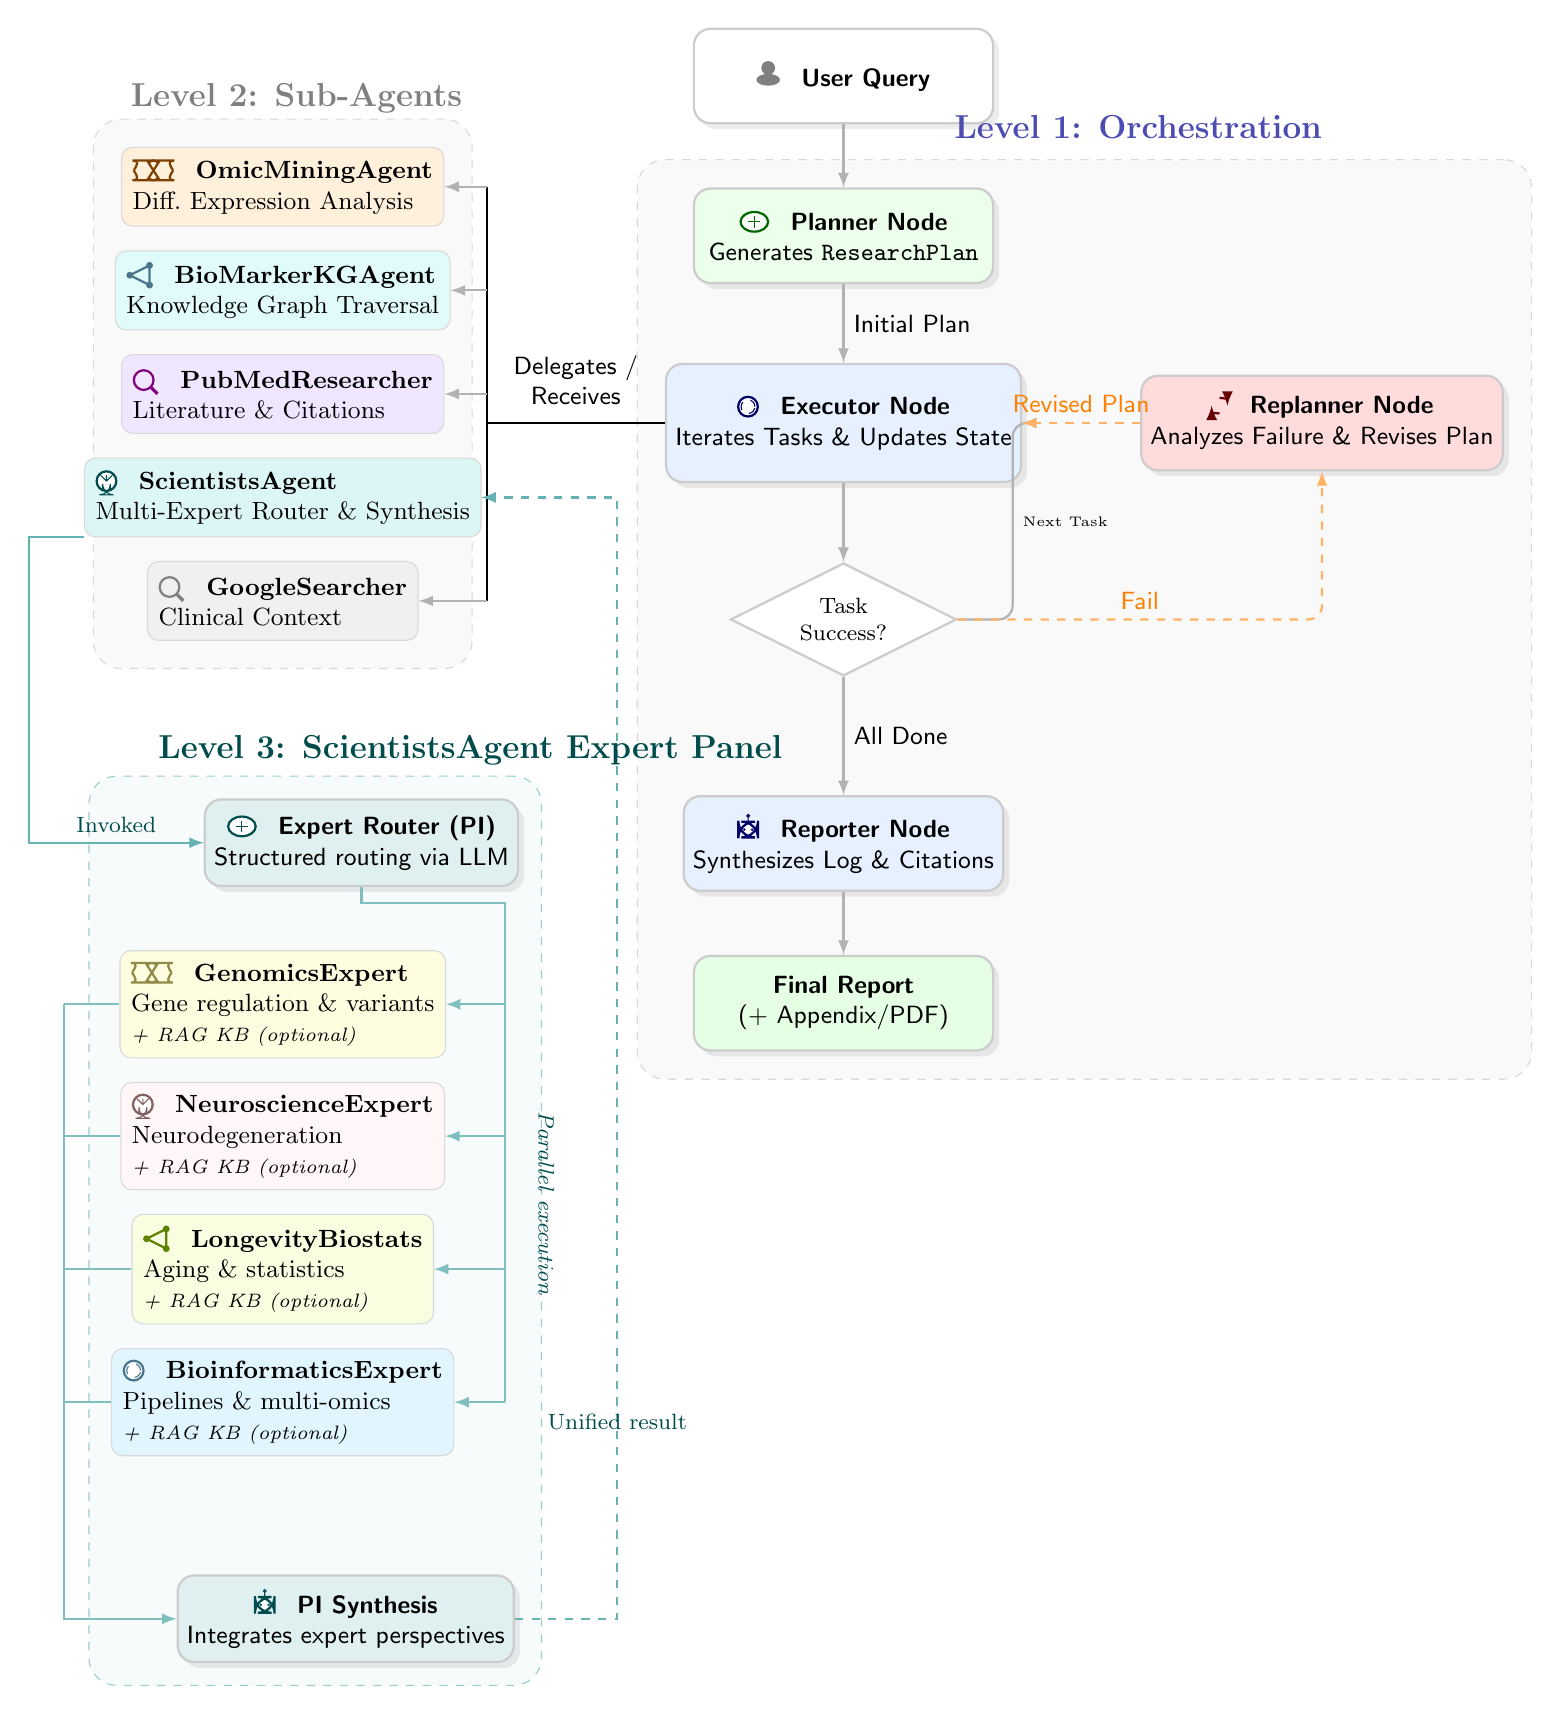
\begin{tikzpicture}[
    font=\sffamily\small,
    >=latex,
    node distance=0.8cm and 1.2cm,
    % --- STYLES (same as original 2-level diagram) ---
    process/.style={
        rectangle, rounded corners=6pt, draw=gray!40, thick,
        minimum width=3.8cm, minimum height=1.2cm, align=center,
        drop shadow={opacity=0.15}
    },
    subagent/.style={
        rectangle, rounded corners=4pt, draw=gray!30,
        minimum width=3.4cm, minimum height=1.0cm, align=left,
        font=\small, inner sep=4pt
    },
    expert/.style={
        rectangle, rounded corners=4pt, draw=gray!30,
        minimum width=3.2cm, minimum height=1.0cm, align=left,
        font=\small, inner sep=4pt
    },
    decision/.style={
        diamond, aspect=2, draw=gray!40, thick, fill=white,
        minimum width=2.5cm, align=center, font=\footnotesize
    },
    arrow/.style={->, thick, draw=gray!60, rounded corners=5pt},
    looparrow/.style={->, thick, draw=orange!60, dashed, rounded corners=5pt},
    groupbox/.style={
        draw=gray!30, dashed, rounded corners=10pt, fill=gray!5, inner sep=10pt
    },
    expertbox/.style={
        draw=teal!40, dashed, rounded corners=10pt, fill=teal!3, inner sep=8pt
    }
]

% ================= LEVEL 1: ORCHESTRATOR =================

% 1. Input
\node[process, fill=white] (start) {\iconUser{gray} \enskip \textbf{User Query}};

% 2. Planner
\node[process, fill=planGreen, below=0.8cm of start] (planner) {
    \iconBrain{green!40!black} \enskip \textbf{Planner Node}\\
     Generates \texttt{ResearchPlan}
};

% 3. Executor
\node[process, fill=orchBlue, below=1.0cm of planner, minimum height=1.5cm] (executor) {
    \iconGears{blue!40!black} \enskip \textbf{Executor Node}\\
    Iterates Tasks \& Updates State
};

% 4. Decision
\node[decision, below=1.0cm of executor] (check) {Task\\Success?};

% 5. Replanner
\node[process, fill=failRed, right=1.5cm of executor] (replanner) {
    \iconCycle{red!40!black} \enskip \textbf{Replanner Node}\\
     Analyzes Failure \& Revises Plan
};

% 6. Reporter
\node[process, fill=orchBlue, below=1.5cm of check] (reporter) {
    \iconRobot{blue!40!black} \enskip \textbf{Reporter Node}\\
    Synthesizes Log \& Citations
};

% 7. Output
\node[process, fill=green!10, below=0.8cm of reporter] (output) {\textbf{Final Report} \\  (+ Appendix/PDF)};

% ================= LEVEL 2: SUB-AGENTS =================

\node[subagent, fill=agentOrange, left=2.8cm of executor, yshift=3.0cm] (ag_omic)
    {\iconDNA{orange!50!black} \enskip \textbf{OmicMiningAgent}\\  Diff.\ Expression Analysis};

\node[subagent, fill=agentCyan, below=0.3cm of ag_omic] (ag_kg)
    {\iconGraph{cyan!50!black} \enskip \textbf{BioMarkerKGAgent}\\  Knowledge Graph Traversal};

\node[subagent, fill=agentPurple, below=0.3cm of ag_kg] (ag_pm)
    {\iconSearch{violet} \enskip \textbf{PubMedResearcher}\\ Literature \& Citations};

\node[subagent, fill=agentTeal, below=0.3cm of ag_pm] (ag_sci)
    {\iconBulb{teal!60!black} \enskip \textbf{ScientistsAgent}\\  Multi-Expert Router \& Synthesis};

\node[subagent, fill=googleGray, below=0.3cm of ag_sci] (ag_goog)
    {\iconSearch{gray} \enskip \textbf{GoogleSearcher}\\  Clinical Context};

% ================= LEVEL 1 CONNECTIONS =================

% Flow Down
\draw[arrow] (start) -- (planner);
\draw[arrow] (planner) -- node[right] {Initial Plan} (executor);
\draw[arrow] (executor) -- (check);

% Success Path
\draw[arrow] (check.south) -- node[right] {All Done} (reporter);
\draw[arrow] (check.east) -- ++(0.7,0) |- node[pos=0.25, right, font=\tiny] {Next Task} (executor.east);

% Failure Loop
\draw[looparrow] (check.east) -| node[pos=0.25, above, color=orange] {Fail} (replanner.south);
\draw[looparrow] (replanner.west) -- node[above,color=orange] {Revised Plan} (executor.east);

% Executor <-> Sub-agent Bus (same spine pattern as original)
\coordinate (spine) at ($(ag_omic.east)!0.5!(ag_goog.east) + (0.7cm, 0)$);

\draw[thick] (executor.west) -- node[above, align=center, yshift=0.1cm]
    {Delegates / \\ Receives} (executor.west -| spine);
\draw[thick] (spine |- ag_omic.east) -- (spine |- ag_goog.east);

\foreach \agent in {ag_omic, ag_kg, ag_pm, ag_sci, ag_goog} {
    \draw[arrow, thick] (spine |- \agent.east) -- (\agent.east);
}

% Final
\draw[arrow] (reporter) -- (output);


% ================= LEVEL 3: EXPERT PANEL (vertical layout) =================

% Router node (below Level 2, shifted right toward center)
\node[process, fill=teal!12, minimum width=3.5cm, minimum height=1.1cm,
      below=2.0cm of ag_goog, xshift=1.0cm] (router)
    {\iconBrain{teal!60!black} \enskip \textbf{Expert Router (PI)}\\
     Structured routing via LLM};

% Four domain experts stacked vertically (like Level 2 sub-agents)
\node[expert, fill=yellow!12, below=0.8cm of router, xshift=-1.0cm] (exp_gen)
    {\iconDNA{yellow!50!black} \enskip \textbf{GenomicsExpert}\\
     Gene regulation \& variants\\
     {\scriptsize\textit{+ RAG KB (optional)}}};

\node[expert, fill=pink!12, below=0.3cm of exp_gen] (exp_neuro)
    {\iconBulb{pink!50!black} \enskip \textbf{NeuroscienceExpert}\\
     Neurodegeneration\\
     {\scriptsize\textit{+ RAG KB (optional)}}};

\node[expert, fill=lime!12, below=0.3cm of exp_neuro] (exp_long)
    {\iconGraph{lime!50!black} \enskip \textbf{LongevityBiostats}\\
     Aging \& statistics\\
     {\scriptsize\textit{+ RAG KB (optional)}}};

\node[expert, fill=cyan!12, below=0.3cm of exp_long] (exp_bio)
    {\iconGears{cyan!50!black} \enskip \textbf{BioinformaticsExpert}\\
     Pipelines \& multi-omics\\
     {\scriptsize\textit{+ RAG KB (optional)}}};

% Synthesis node (below experts, with more spacing)
\node[process, fill=teal!12, minimum width=3.5cm, minimum height=1.1cm,
      below=1.5cm of exp_bio, xshift=0.8cm] (synth)
    {\iconRobot{teal!60!black} \enskip \textbf{PI Synthesis}\\
     Integrates expert perspectives};

% --- Level 3 connections ---

% ScientistsAgent -> Router (clean route down the left side)
\coordinate (sci_drop) at ($(ag_sci.south west) + (-0.7cm, 0)$);
\draw[->, thick, draw=teal!60]
    (ag_sci.south west) -- (sci_drop) -- (sci_drop |- router.west) -- (router.west)
    node[pos=0.5, above, font=\footnotesize, color=teal!60!black] {Invoked};

% Router -> Experts: spine bus (right side of experts, like Level 2)
\coordinate (l3spine) at ($(exp_gen.east)!0.5!(exp_bio.east) + (0.7cm, 0)$);
\draw[thick, draw=teal!50] (router.south) -- ++(0,-0.2) -| (l3spine |- exp_gen.east);
\draw[thick, draw=teal!50] (l3spine |- exp_gen.east) -- (l3spine |- exp_bio.east);
\foreach \exp in {exp_gen, exp_neuro, exp_long, exp_bio} {
    \draw[->, thick, draw=teal!50] (l3spine |- \exp.east) -- (\exp.east);
}

% Annotation next to spine
\node[color=teal!60!black, font=\footnotesize\itshape, rotate=-90, anchor=south]
    at ($(l3spine) + (0.3cm, 0)$) {Parallel execution};

% Experts -> Synthesis: spine bus (left side of experts)
\coordinate (l3spineL) at ($(exp_gen.west) + (-0.7cm, 0)$);
\draw[thick, draw=teal!50] (l3spineL |- exp_gen.west) -- (l3spineL |- exp_bio.west);
\foreach \exp in {exp_gen, exp_neuro, exp_long, exp_bio} {
    \draw[thick, draw=teal!50] (\exp.west) -- (l3spineL |- \exp.west);
}
\draw[->, thick, draw=teal!50] (l3spineL |- exp_bio.west) -- (l3spineL |- synth.west) -- (synth.west);

% Return path: Synthesis -> back up to ScientistsAgent
\coordinate (return_r) at ($(synth.east) + (1.3cm, 0)$);
\draw[->, thick, draw=teal!60, dashed]
    (synth.east) -- (return_r) |- (ag_sci.east)
    node[pos=0.08, above, font=\footnotesize, color=teal!60!black] {Unified result};

% ================= GROUP BOXES & LABELS =================

% Level 1 label & box
\node[anchor=south west, font=\bfseries\large, color=blue!40!gray]
    at ($(planner.north west)+(3.2,0.5)$) {Level 1: Orchestration};
\begin{scope}[on background layer]
    \node[groupbox, fit=(planner) (executor) (replanner) (reporter) (check) (output)] {};
\end{scope}

% Level 2 label & box
\node[anchor=south west, font=\bfseries\large, color=gray]
    at ($(ag_omic.north west)+(0,0.3)$) {Level 2: Sub-Agents};
\begin{scope}[on background layer]
    \node[groupbox, fit=(ag_omic) (ag_goog)] {};
\end{scope}

% Level 3 label & box
\node[anchor=south west, font=\bfseries\large, color=teal!60!black]
    at ($(router.north west)+(-0.7,0.3)$) {Level 3: ScientistsAgent Expert Panel};
\begin{scope}[on background layer]
    \node[expertbox, fit=(router) (exp_gen) (exp_bio) (synth)] {};
\end{scope}

\end{tikzpicture}%
}% end resizebox
\caption{Three-level architecture of OmniCellAgent. 
\textbf{Level~1 (Orchestration):} A Planner decomposes the user query into a 
\texttt{ResearchPlan}; the Executor dispatches each task to the appropriate 
sub-agent, a Decision node triggers the Replanner on failure, and the Reporter 
compiles the final synthesis with citations. 
\textbf{Level~2 (Sub-Agents):} Five specialised sub-agents—OmicMiningAgent, 
BioMarkerKGAgent, PubMedResearcher, ScientistsAgent, and GoogleSearcher—are 
invoked in parallel or sequentially by the Executor. 
\textbf{Level~3 (Expert Panel):} Inside ScientistsAgent, an Expert Router (PI) 
performs structured LLM-based routing to four domain experts (Genomics, 
Neuroscience, Longevity/Biostatistics, Bioinformatics), each optionally backed 
by a RAG knowledge base; a PI Synthesis node integrates expert perspectives 
and returns a unified result.}
\label{fig:architecture}
\end{figure}

\end{document}
